% Options for packages loaded elsewhere
\PassOptionsToPackage{unicode}{hyperref}
\PassOptionsToPackage{hyphens}{url}
\PassOptionsToPackage{dvipsnames,svgnames,x11names}{xcolor}
%
\documentclass[
]{article}
\usepackage{amsmath,amssymb}
\usepackage{iftex}
\ifPDFTeX
  \usepackage[T1]{fontenc}
  \usepackage[utf8]{inputenc}
  \usepackage{textcomp} % provide euro and other symbols
\else % if luatex or xetex
  \usepackage{unicode-math} % this also loads fontspec
  \defaultfontfeatures{Scale=MatchLowercase}
  \defaultfontfeatures[\rmfamily]{Ligatures=TeX,Scale=1}
\fi
\usepackage{lmodern}
\ifPDFTeX\else
  % xetex/luatex font selection
\fi
% Use upquote if available, for straight quotes in verbatim environments
\IfFileExists{upquote.sty}{\usepackage{upquote}}{}
\IfFileExists{microtype.sty}{% use microtype if available
  \usepackage[]{microtype}
  \UseMicrotypeSet[protrusion]{basicmath} % disable protrusion for tt fonts
}{}
\makeatletter
\@ifundefined{KOMAClassName}{% if non-KOMA class
  \IfFileExists{parskip.sty}{%
    \usepackage{parskip}
  }{% else
    \setlength{\parindent}{0pt}
    \setlength{\parskip}{6pt plus 2pt minus 1pt}}
}{% if KOMA class
  \KOMAoptions{parskip=half}}
\makeatother
\usepackage{xcolor}
\usepackage[margin = 0.5in]{geometry}
\usepackage{color}
\usepackage{fancyvrb}
\newcommand{\VerbBar}{|}
\newcommand{\VERB}{\Verb[commandchars=\\\{\}]}
\DefineVerbatimEnvironment{Highlighting}{Verbatim}{commandchars=\\\{\}}
% Add ',fontsize=\small' for more characters per line
\newenvironment{Shaded}{}{}
\newcommand{\AlertTok}[1]{\textcolor[rgb]{1.00,0.00,0.00}{#1}}
\newcommand{\AnnotationTok}[1]{\textcolor[rgb]{0.00,0.50,0.00}{#1}}
\newcommand{\AttributeTok}[1]{#1}
\newcommand{\BaseNTok}[1]{#1}
\newcommand{\BuiltInTok}[1]{#1}
\newcommand{\CharTok}[1]{\textcolor[rgb]{0.00,0.50,0.50}{#1}}
\newcommand{\CommentTok}[1]{\textcolor[rgb]{0.00,0.50,0.00}{#1}}
\newcommand{\CommentVarTok}[1]{\textcolor[rgb]{0.00,0.50,0.00}{#1}}
\newcommand{\ConstantTok}[1]{#1}
\newcommand{\ControlFlowTok}[1]{\textcolor[rgb]{0.00,0.00,1.00}{#1}}
\newcommand{\DataTypeTok}[1]{#1}
\newcommand{\DecValTok}[1]{#1}
\newcommand{\DocumentationTok}[1]{\textcolor[rgb]{0.00,0.50,0.00}{#1}}
\newcommand{\ErrorTok}[1]{\textcolor[rgb]{1.00,0.00,0.00}{\textbf{#1}}}
\newcommand{\ExtensionTok}[1]{#1}
\newcommand{\FloatTok}[1]{#1}
\newcommand{\FunctionTok}[1]{#1}
\newcommand{\ImportTok}[1]{#1}
\newcommand{\InformationTok}[1]{\textcolor[rgb]{0.00,0.50,0.00}{#1}}
\newcommand{\KeywordTok}[1]{\textcolor[rgb]{0.00,0.00,1.00}{#1}}
\newcommand{\NormalTok}[1]{#1}
\newcommand{\OperatorTok}[1]{#1}
\newcommand{\OtherTok}[1]{\textcolor[rgb]{1.00,0.25,0.00}{#1}}
\newcommand{\PreprocessorTok}[1]{\textcolor[rgb]{1.00,0.25,0.00}{#1}}
\newcommand{\RegionMarkerTok}[1]{#1}
\newcommand{\SpecialCharTok}[1]{\textcolor[rgb]{0.00,0.50,0.50}{#1}}
\newcommand{\SpecialStringTok}[1]{\textcolor[rgb]{0.00,0.50,0.50}{#1}}
\newcommand{\StringTok}[1]{\textcolor[rgb]{0.00,0.50,0.50}{#1}}
\newcommand{\VariableTok}[1]{#1}
\newcommand{\VerbatimStringTok}[1]{\textcolor[rgb]{0.00,0.50,0.50}{#1}}
\newcommand{\WarningTok}[1]{\textcolor[rgb]{0.00,0.50,0.00}{\textbf{#1}}}
\usepackage{longtable,booktabs,array}
\usepackage{calc} % for calculating minipage widths
% Correct order of tables after \paragraph or \subparagraph
\usepackage{etoolbox}
\makeatletter
\patchcmd\longtable{\par}{\if@noskipsec\mbox{}\fi\par}{}{}
\makeatother
% Allow footnotes in longtable head/foot
\IfFileExists{footnotehyper.sty}{\usepackage{footnotehyper}}{\usepackage{footnote}}
\makesavenoteenv{longtable}
\usepackage{graphicx}
\makeatletter
\newsavebox\pandoc@box
\newcommand*\pandocbounded[1]{% scales image to fit in text height/width
  \sbox\pandoc@box{#1}%
  \Gscale@div\@tempa{\textheight}{\dimexpr\ht\pandoc@box+\dp\pandoc@box\relax}%
  \Gscale@div\@tempb{\linewidth}{\wd\pandoc@box}%
  \ifdim\@tempb\p@<\@tempa\p@\let\@tempa\@tempb\fi% select the smaller of both
  \ifdim\@tempa\p@<\p@\scalebox{\@tempa}{\usebox\pandoc@box}%
  \else\usebox{\pandoc@box}%
  \fi%
}
% Set default figure placement to htbp
\def\fps@figure{htbp}
\makeatother
\setlength{\emergencystretch}{3em} % prevent overfull lines
\providecommand{\tightlist}{%
  \setlength{\itemsep}{0pt}\setlength{\parskip}{0pt}}
\setcounter{secnumdepth}{5}
\usepackage{booktabs}
\usepackage{longtable}
\usepackage{array}
\usepackage{multirow}
\usepackage{wrapfig}
\usepackage{float}
\usepackage{colortbl}
\usepackage{pdflscape}
\usepackage{tabu}
\usepackage{threeparttable}
\usepackage{threeparttablex}
\usepackage[normalem]{ulem}
\usepackage{makecell}
\usepackage{xcolor}
\usepackage{booktabs}
\usepackage{longtable}
\usepackage{array}
\usepackage{multirow}
\usepackage{wrapfig}
\usepackage{float}
\usepackage{colortbl}
\usepackage{pdflscape}
\usepackage{tabu}
\usepackage{threeparttable}
\usepackage{threeparttablex}
\usepackage[normalem]{ulem}
\usepackage{makecell}
\usepackage{xcolor}
\usepackage{bookmark}
\IfFileExists{xurl.sty}{\usepackage{xurl}}{} % add URL line breaks if available
\urlstyle{same}
\hypersetup{
  pdftitle={Crime Information Report on the District Of Columbia in 2017(Washington DC)},
  pdfauthor={Logan Salinas},
  colorlinks=true,
  linkcolor={Maroon},
  filecolor={Maroon},
  citecolor={Blue},
  urlcolor={blue},
  pdfcreator={LaTeX via pandoc}}

\title{Crime Information Report on the District Of Columbia in
2017(Washington DC)}
\author{Logan Salinas}
\date{August 14, 2025}

\begin{document}
\maketitle

\clearpage

\section{Background}\label{background}

The research that I will be conducting will revolve around the crimes
committed as well as the crimes reported in the United States Capital,
Washington DC. I will be responsible on identifying any trends or
patterns that is within data set containing crime reports in Washington
DC. Specifically, I look into the type of offense that was committed and
when the crime was reported. I'm hoping by the end of my research, I'll
be able to answer the to the points mentioned above and give people a
good understanding of where in D.C. the most crimes are committed and
hopefully help them avoid those areas if they were ever to come visit
Washington DC one day.

\subsection{Description of Data}\label{description-of-data}

The data that I'll be using today is a csv file called
\texttt{Crime\_incidents\_in\_2017.csv}. I got this data from data.gov
which is a United States open government website. This website allows
the public to access data regarding anything that has to something or is
associated with the U.S. government. The data that I'm using is
information regarding crime reports in Washington D.C. in the year 2017.
Some important things on the csv file are the variables and
observations. The data that I'm handling here has around 33,000 rows of
data/observations and 27 variables/columns. So I have to be extra
careful when I utilize data manipulation.

\subsubsection{Data Dictionary}\label{data-dictionary}

\begin{itemize}
\tightlist
\item
  \textbf{REPORT\_DAT:} The Date in time in which the crime was
  reported.
\item
  \textbf{SHIFT:} The police shift during which the crime occurred.
\item
  \textbf{OFFENSE:} Type of crime committed based on the report.
\item
  \textbf{LONGITUDE/LATITUDE:} The coordinates of where the crime
  happened.
\item
  \textbf{Month:} The month in which the crime was reported.
\item
  \textbf{Hour:} The hour in which the crime was reported.
\end{itemize}

\subsection{Summary Table of Crimes Reported Each Month per Offense
(Bivariate
Aggregation)}\label{summary-table-of-crimes-reported-each-month-per-offense-bivariate-aggregation}

We are exploring the the possible relationship between Month in which
the crime was reported and the type of offense in the report itself, the
two variables \texttt{Month} and \texttt{OFFENSE} are categorical. By
using the \texttt{Crime\_Incidents\_in\_2017.csv} data set, we are able
to display a table of the type of offenses that was reported in each
month and identify a pattern if certain type of offenses are being
committed more than others on a certain month.

\begin{table}[!h]
\centering
\caption{\label{tab:appendix-load-wide-summary-table}Total Amount of Crimes Reported Each Month per Offense}
\centering
\resizebox{\ifdim\width>\linewidth\linewidth\else\width\fi}{!}{
\begin{tabular}[t]{l|r|r|r|r|r|r|r|r|r}
\hline
Month & ARSON & ASSAULT W/DANGEROUS WEAPON & BURGLARY & HOMICIDE & MOTOR VEHICLE THEFT & ROBBERY & SEX ABUSE & THEFT F/AUTO & THEFT/OTHER\\
\hline
Jan & 1 & 183 & 154 & 8 & 170 & 209 & 22 & 1098 & 1160\\
\hline
Feb & 0 & 148 & 104 & 6 & 165 & 155 & 22 & 734 & 1087\\
\hline
Mar & 0 & 131 & 117 & 14 & 173 & 138 & 24 & 661 & 1068\\
\hline
Apr & 2 & 160 & 138 & 7 & 209 & 170 & 28 & 799 & 1183\\
\hline
May & 0 & 158 & 141 & 8 & 214 & 148 & 34 & 1051 & 1310\\
\hline
Jun & 1 & 154 & 124 & 11 & 222 & 188 & 29 & 889 & 1250\\
\hline
Jul & 0 & 169 & 128 & 12 & 250 & 197 & 24 & 823 & 1271\\
\hline
Aug & 1 & 157 & 120 & 8 & 228 & 187 & 35 & 826 & 1278\\
\hline
Sep & 0 & 160 & 130 & 10 & 193 & 187 & 20 & 821 & 1292\\
\hline
Oct & 0 & 152 & 130 & 11 & 198 & 231 & 24 & 912 & 1292\\
\hline
Nov & 0 & 141 & 125 & 9 & 176 & 195 & 14 & 809 & 1194\\
\hline
Dec & 0 & 138 & 119 & 11 & 209 & 164 & 21 & 833 & 1079\\
\hline
\end{tabular}}
\end{table}

The bar plot that is going to be displayed below will give us an idea of
how many times a certain offense was reported at a certain month. I
believe that using a bar plot here is appropriate because it will give
us a plot of results for the number of crimes reported each month, and
the amount of offenses in each of those reports.

\begin{center}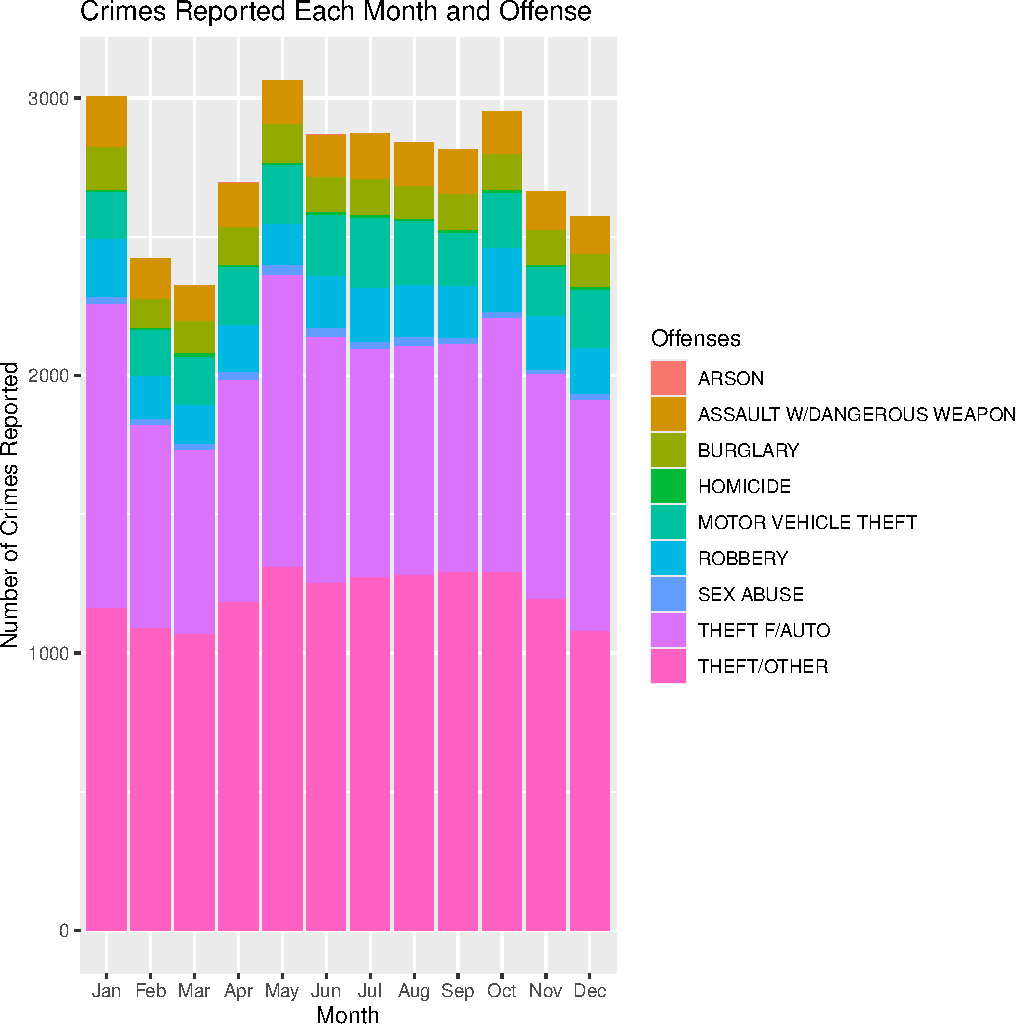
\includegraphics{./figures/appendix-plot-bar-graph-1} \end{center}

\subsubsection{Discussion}\label{discussion}

The table gave us an idea of how many type of offenses were reported for
every month of the year 2017. By the looks of it, one of the type of
crimes, arson, is rarely reported. The results of the stacked bar plot
show that the majority of crimes that were reported in Washington DC
were crimes related to theft, and auto theft. There isn't a month that
stands out by a huge margin where I can say that a particular month is
known for having the highest amount of reports on a certain offense. But
what I can say is that theft and auto theft offenses increased during
the middle of the year (May, June, July). All other offenses are around
similar amounts for each month.

\clearpage

\section{Geographic Summary of Crime Coordinates (Univariate
Aggregation)}\label{geographic-summary-of-crime-coordinates-univariate-aggregation}

What we are doing is using the \texttt{longitude} and \texttt{latitude}
variables to find where exactly these crimes are being reported in
Washington DC as well as the type of crime that took place in that area.
For the univariate summary table, I display the minimum, maximum, mean,
median, and standard deviation values of the longitude and latitude.
These values will help is in finding where exactly in Washington DC does
reported crime happen the most in.

\begin{longtable}[]{@{}lr@{}}
\caption{Univariate Summary Table of Longitude and
Latitude}\tabularnewline
\toprule\noalign{}
name & value \\
\midrule\noalign{}
\endfirsthead
\toprule\noalign{}
name & value \\
\midrule\noalign{}
\endhead
\bottomrule\noalign{}
\endlastfoot
longitude\_min & -77.1123165 \\
longitude\_max & -76.9100205 \\
longitude\_mean & -77.0069839 \\
longitude\_median & -77.0106764 \\
longitude\_sd & 0.0363280 \\
latitude\_min & 38.8134705 \\
latitude\_max & 38.9935598 \\
latitude\_mean & 38.9064802 \\
latitude\_median & 38.9060616 \\
latitude\_sd & 0.0302385 \\
\end{longtable}

For this plot, I ended up doing a scatter plot, the reasoning beheind
this is that we are dealing with longitude and latitude values. We can
treat the scatter plot grid as like a map and use the variables stated
previous to pin point the where exactly what type of crime was report.
What's very interesting about the scatter plot is that it outline the
boarders of Washington D.C..

\begin{center}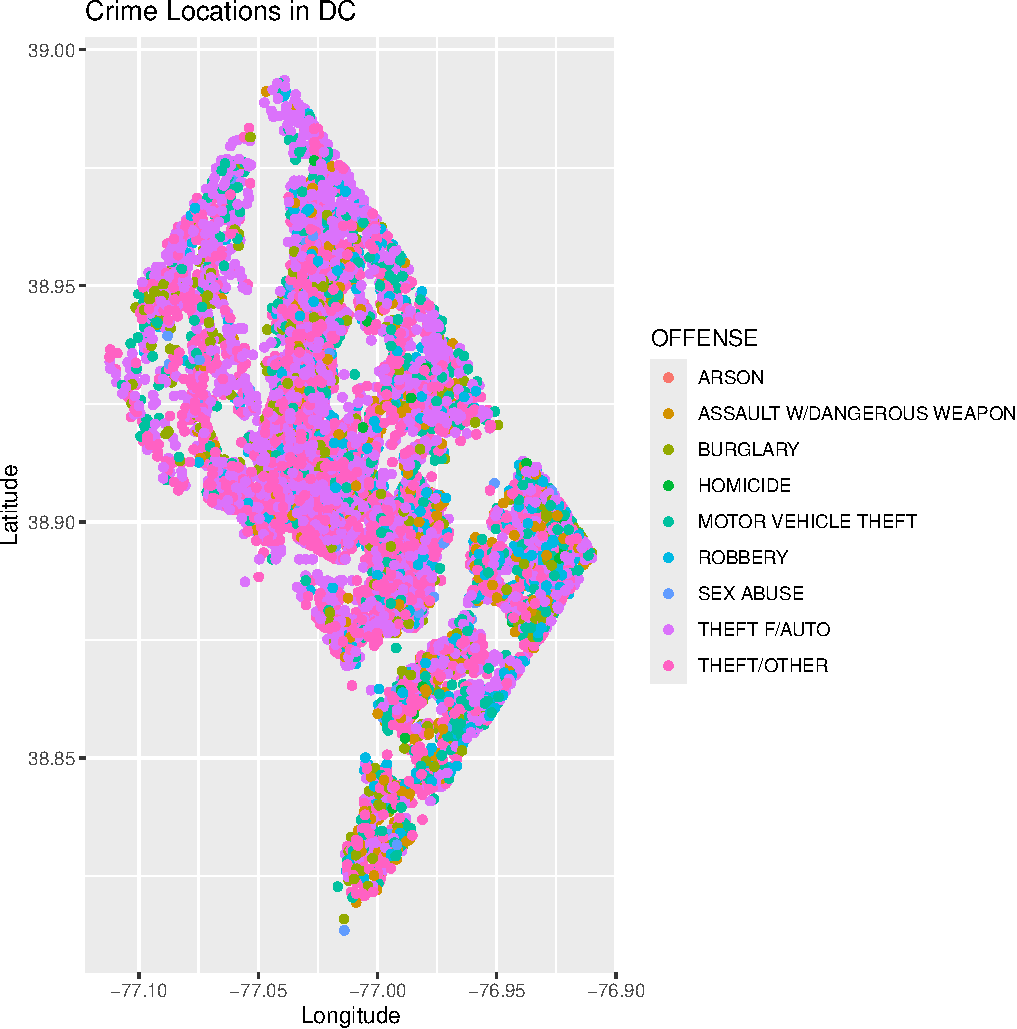
\includegraphics{./figures/appendix-plot-scatterplot-1} \end{center}

\subsubsection{Discusion on Scatter
plot}\label{discusion-on-scatter-plot}

From the table, we were able to obtain the summary statistics of the
longitude and latitude variables. Nothing really stood out in the table.
If we took the mean of the longitude and latitude and put them together,
then we would get the average coordinates of where crimes are reported.

As stated before, the points on the scatter plot outline the boarder of
Washington DC. And based off the amount of color points plotted on the
scatter plot, we can say that the majority crimes that happen in the
central part of D.C. is Theft, and behind Theft is auto Theft and
Robbery. This information helps further prove our question above about
certain offenses being reported more in certain parts of D.C. compared
to others.

\section{Summary Table of Hours For Each Shift (Bivariate
Aggregation)}\label{summary-table-of-hours-for-each-shift-bivariate-aggregation}

For this table and plot we are exploring the relationship between the
hours that a report was made and the police shift during which the crime
was reported. We use the \texttt{crime\_incidents\_df} data set to find
the minimum, lower quantile, median, upper quantile, maximum, mean, and
standard deviation of the hour of the report for every shift. This table
will give us a better understanding of crimes being reported at certain
hours of the day and the shift that documents these crimes.

\begin{longtable}[]{@{}
  >{\raggedright\arraybackslash}p{(\linewidth - 14\tabcolsep) * \real{0.0918}}
  >{\raggedleft\arraybackslash}p{(\linewidth - 14\tabcolsep) * \real{0.0918}}
  >{\raggedleft\arraybackslash}p{(\linewidth - 14\tabcolsep) * \real{0.2041}}
  >{\raggedleft\arraybackslash}p{(\linewidth - 14\tabcolsep) * \real{0.1224}}
  >{\raggedleft\arraybackslash}p{(\linewidth - 14\tabcolsep) * \real{0.2041}}
  >{\raggedleft\arraybackslash}p{(\linewidth - 14\tabcolsep) * \real{0.0918}}
  >{\raggedleft\arraybackslash}p{(\linewidth - 14\tabcolsep) * \real{0.1020}}
  >{\raggedleft\arraybackslash}p{(\linewidth - 14\tabcolsep) * \real{0.0918}}@{}}
\caption{Bivariate Summary Table of Hours per Shift}\tabularnewline
\toprule\noalign{}
\begin{minipage}[b]{\linewidth}\raggedright
SHIFT
\end{minipage} & \begin{minipage}[b]{\linewidth}\raggedleft
min\_hour
\end{minipage} & \begin{minipage}[b]{\linewidth}\raggedleft
lower\_quantile\_hour
\end{minipage} & \begin{minipage}[b]{\linewidth}\raggedleft
median\_hour
\end{minipage} & \begin{minipage}[b]{\linewidth}\raggedleft
upper\_quantile\_hour
\end{minipage} & \begin{minipage}[b]{\linewidth}\raggedleft
max\_hour
\end{minipage} & \begin{minipage}[b]{\linewidth}\raggedleft
mean\_hour
\end{minipage} & \begin{minipage}[b]{\linewidth}\raggedleft
sd\_hour
\end{minipage} \\
\midrule\noalign{}
\endfirsthead
\toprule\noalign{}
\begin{minipage}[b]{\linewidth}\raggedright
SHIFT
\end{minipage} & \begin{minipage}[b]{\linewidth}\raggedleft
min\_hour
\end{minipage} & \begin{minipage}[b]{\linewidth}\raggedleft
lower\_quantile\_hour
\end{minipage} & \begin{minipage}[b]{\linewidth}\raggedleft
median\_hour
\end{minipage} & \begin{minipage}[b]{\linewidth}\raggedleft
upper\_quantile\_hour
\end{minipage} & \begin{minipage}[b]{\linewidth}\raggedleft
max\_hour
\end{minipage} & \begin{minipage}[b]{\linewidth}\raggedleft
mean\_hour
\end{minipage} & \begin{minipage}[b]{\linewidth}\raggedleft
sd\_hour
\end{minipage} \\
\midrule\noalign{}
\endhead
\bottomrule\noalign{}
\endlastfoot
DAY & 11 & 14 & 16 & 17 & 20 & 15.543717 & 2.181546 \\
EVENING & 0 & 1 & 19 & 22 & 23 & 12.454643 & 9.990945 \\
MIDNIGHT & 3 & 4 & 6 & 8 & 12 & 6.181396 & 2.357499 \\
\end{longtable}

For this part, I decided to use a bar plot because the use of a bar plot
would help us find the hours crimes that are reported during a certain
police shift.

\begin{center}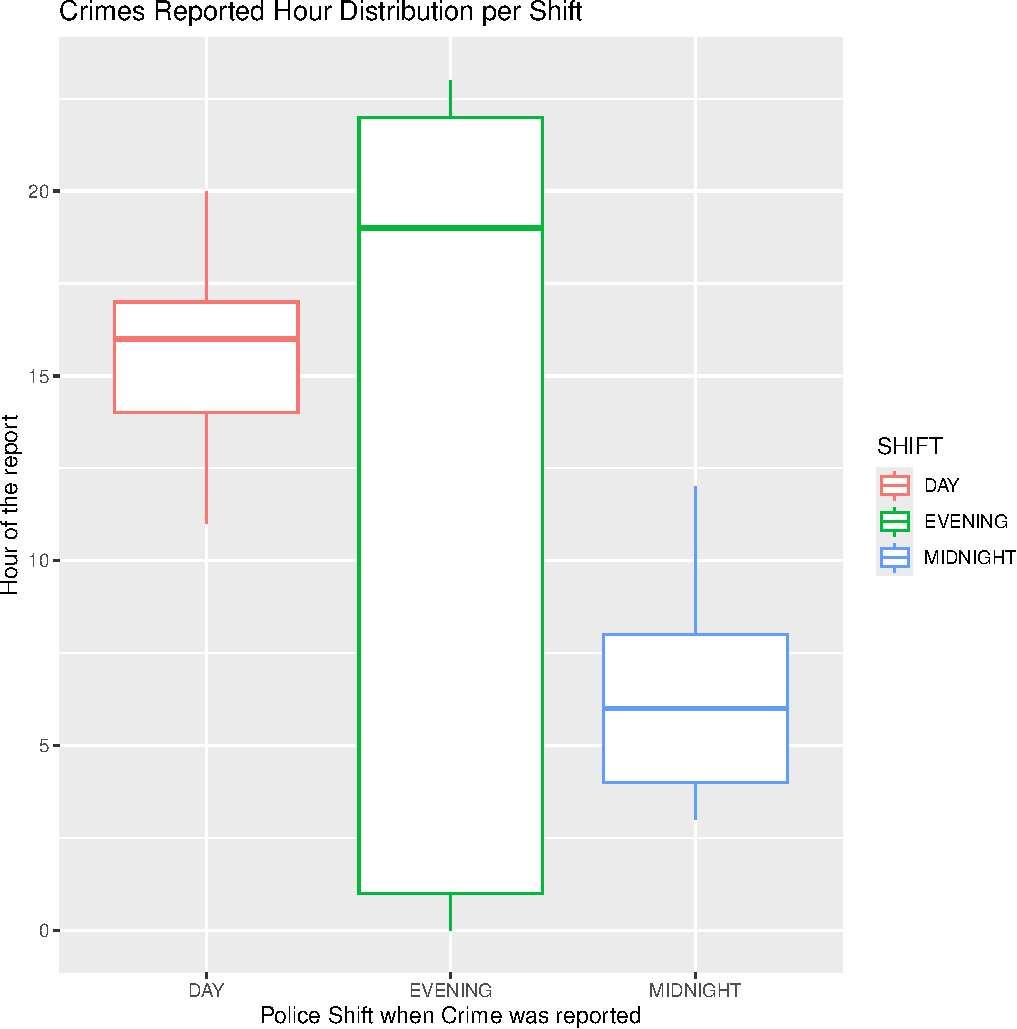
\includegraphics{./figures/appendix-plot-boxplot-1} \end{center}

\subsubsection{Discussion on Box plot}\label{discussion-on-box-plot}

The table gives us information regarding when crimes are reported during
certain hours of the day for every shift. One issue that I have with the
table is the min\_hour for the evening shift. I asked myself how is
crime reported at the early hours of the morning considered a report
done during the evening shift?

As we can see in the box plot, crimes reported during the day shift are
usually reported during the afternoon hours, crimes reported during the
evening shift are usually reported almost all hours of the day, and
crimes reported during the midnight shift are usually reported during
the early hours of the morning. With this information, we know have an
idea of what hours of the day are reported to each shift.

\section{Summary Table of Number of Reports for Each Shift (Bivariate
Aggregation)}\label{summary-table-of-number-of-reports-for-each-shift-bivariate-aggregation}

Finally, we are exploring the the relationship between the months and
the number of crimes reported for each police shift. We first use
\texttt{crime\_incidents\_df} data set to find the summary statistics of
the number of crimes reported per shift. This information will give us
an idea of which shifts had the most or least number of crimes reported.
It will also help us visualize the trend for crimes reported per shift
based on the months.

\begin{longtable}[]{@{}
  >{\raggedright\arraybackslash}p{(\linewidth - 10\tabcolsep) * \real{0.1250}}
  >{\raggedleft\arraybackslash}p{(\linewidth - 10\tabcolsep) * \real{0.1667}}
  >{\raggedleft\arraybackslash}p{(\linewidth - 10\tabcolsep) * \real{0.1667}}
  >{\raggedleft\arraybackslash}p{(\linewidth - 10\tabcolsep) * \real{0.1806}}
  >{\raggedleft\arraybackslash}p{(\linewidth - 10\tabcolsep) * \real{0.2083}}
  >{\raggedleft\arraybackslash}p{(\linewidth - 10\tabcolsep) * \real{0.1528}}@{}}
\caption{Bivariate Summary Table of Reports per Shift}\tabularnewline
\toprule\noalign{}
\begin{minipage}[b]{\linewidth}\raggedright
SHIFT
\end{minipage} & \begin{minipage}[b]{\linewidth}\raggedleft
min\_reports
\end{minipage} & \begin{minipage}[b]{\linewidth}\raggedleft
max\_reports
\end{minipage} & \begin{minipage}[b]{\linewidth}\raggedleft
mean\_reports
\end{minipage} & \begin{minipage}[b]{\linewidth}\raggedleft
median\_reports
\end{minipage} & \begin{minipage}[b]{\linewidth}\raggedleft
sd\_reports
\end{minipage} \\
\midrule\noalign{}
\endfirsthead
\toprule\noalign{}
\begin{minipage}[b]{\linewidth}\raggedright
SHIFT
\end{minipage} & \begin{minipage}[b]{\linewidth}\raggedleft
min\_reports
\end{minipage} & \begin{minipage}[b]{\linewidth}\raggedleft
max\_reports
\end{minipage} & \begin{minipage}[b]{\linewidth}\raggedleft
mean\_reports
\end{minipage} & \begin{minipage}[b]{\linewidth}\raggedleft
median\_reports
\end{minipage} & \begin{minipage}[b]{\linewidth}\raggedleft
sd\_reports
\end{minipage} \\
\midrule\noalign{}
\endhead
\bottomrule\noalign{}
\endlastfoot
DAY & 877 & 1135 & 1016.000 & 1036.0 & 81.80798 \\
EVENING & 1010 & 1376 & 1167.583 & 1146.5 & 92.93933 \\
MIDNIGHT & 420 & 671 & 574.250 & 583.5 & 85.03596 \\
\end{longtable}

I decided to use a plot trend line for this part because I believed that
using the plot trend line method would help me answer the question of
``what is the monthly crime trend by shift?'' based on the number of
crimes reported. The plot trend line method would be able to utilize all
three variables to answer that question.

\begin{center}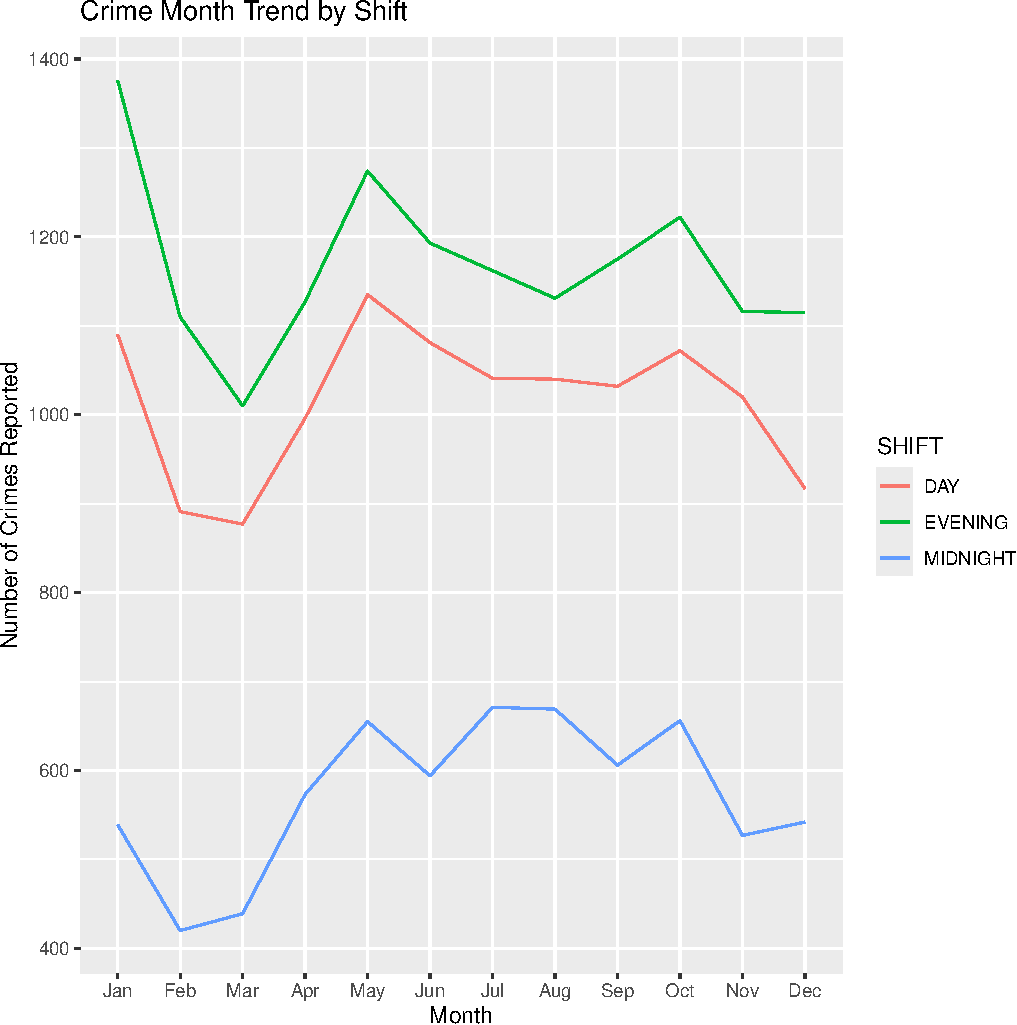
\includegraphics{./figures/appendix-plot-trend-line-1} \end{center}

\subsubsection{Discussion}\label{discussion-1}

From the information of the summary table, Evening shifts receive the
majority amount of crime reported on average, and have received the
highest amount of crimes reported for one month compared to all months
for other shifts. The trend line graph backs up the table information.
As we can see in the plot trend line, the line, that represents the
trend of crimes reported per shift, that is green(Evening shift) is
higher on the graph then the red(Day Shift) or blue(Midnight Shift)
line.

\section{Proposed Research Method and
Questions}\label{proposed-research-method-and-questions}

\begin{enumerate}
\def\labelenumi{\arabic{enumi}.}
\tightlist
\item
  One question that I want to find the answer to is
  \texttt{if\ we\ can\ predict\ the\ type\ of\ offenses\ based\ on\ the\ month,\ hour,\ and\ coordinates\ of\ the\ crime\ report\ given\ to\ us?}
  Since we are given a data of crime reports in Washington DC, we could
  use variables in the data frame and the entries associated with those
  variables as training data. We train the model to understand the
  relationship between pair variables and try to predict the type of
  offenses from new crime reports, which would contain the month, hour,
  longitude and latitude. Since we are trying to predict the type of
  offense that is going to be committed based on a couple of variables,
  the statistical learning technique I am going to use will be
  supervised learning. Utilizing this technique will allow me to learn
  more about the relationship between the time/location and the type of
  offense in each report in the data set. This will help me create and
  train a model that can make predictions on the type of offenses based
  on the time and location mentioned in the crime report, assuming the
  report had a time and location written, but not the type of offense
  committed.
\end{enumerate}

\begin{verbatim}
Call:
multinom(formula = OFFENSE ~ Hour + LONGITUDE + LATITUDE, data = crime_train, 
    family = binomial)

Coefficients:
                           (Intercept)        Hour LONGITUDE    LATITUDE
ASSAULT W/DANGEROUS WEAPON   750.08633 -0.08536744  6.024605  -7.1736749
BURGLARY                     -15.06984 -0.05356940 -2.310996  -4.0155403
HOMICIDE                     109.02404 -0.22044783 -6.493457 -15.5213464
MOTOR VEHICLE THEFT          353.08625 -0.04567103  6.203280   3.3815174
ROBBERY                      161.39056 -0.08961609  2.052821   0.1048833
SEX ABUSE                     71.42175 -0.06241796 -1.727118  -5.1217929
THEFT F/AUTO                -756.90273 -0.03793543 -6.322689   7.1551910
THEFT/OTHER                 -677.68220 -0.04521840 -9.190826  -0.5468664

Std. Errors:
                            (Intercept)       Hour  LONGITUDE    LATITUDE
ASSAULT W/DANGEROUS WEAPON 0.0004868488 0.08346952 0.36926995 0.730480036
BURGLARY                   0.0004162205 0.08348162 0.06944330 0.134826264
HOMICIDE                   0.0001840228 0.08606662 0.01433694 0.008677754
MOTOR VEHICLE THEFT        0.0006291977 0.08345131 0.36655093 0.724939860
ROBBERY                    0.0010927775 0.08345633 0.36904888 0.729975132
SEX ABUSE                  0.0001895192 0.08383249 0.01625894 0.017563178
THEFT F/AUTO               0.0009366610 0.08340620 0.23853626 0.471347030
THEFT/OTHER                0.0012285455 0.08340203 0.21405571 0.422864320

Residual Deviance: 71548.95 
AIC: 71612.95 
\end{verbatim}

\begin{enumerate}
\def\labelenumi{\arabic{enumi}.}
\setcounter{enumi}{1}
\tightlist
\item
  Another research question I could look into is
  \texttt{does\ an\ offense\textquotesingle{}s\ frequency\ vary\ across\ months?}
  From the trend line plot shown earlier in the report, we have already
  answered a third of this question, that being the frequency of crimes
  being reported for each shift by month. The statistical learning
  technique I am going to use to answer this research question will be
  Chi-square test. The null hypotheses will be that the type of offense
  and the month are independent, and the alternative hypotheses will be
  that the type of offense and the month are dependent. The results that
  I get for carrying out the chi-square test will determine whether we
  reject or fail to reject the null hypothesis. If we reject the null
  hypothesis, then both the type of offense and month are dependent,
  which means that there is a pattern/trend. If we fail to reject the
  null hypotheses, then both the type of offense and month are
  independent, which means that there is no pattern/trend.
\end{enumerate}

\begin{verbatim}

    Pearson's Chi-squared test

data:  table_crime
X-squared = 192.8, df = 88, p-value = 8.289e-10
\end{verbatim}

\textbf{Answer to Question 2:} Based on the p value we got after
carrying out the chi-square test, we confidently reject the null
hypothesis. Which means that the type of offense and the month are
dependent on each other which implies that there is a pattern between
the two variables.

\begin{enumerate}
\def\labelenumi{\arabic{enumi}.}
\setcounter{enumi}{2}
\tightlist
\item
  And the last research question I could look into is
  \texttt{Are\ there\ certain\ areas\ in\ Washington\ DC\ where\ certain\ type\ of\ offenses\ are\ reported\ a\ lot\ more\ than\ others?}
  In the data set, there is a latitude and longitude entry in each crime
  report. By using the unsupervised learning method, we can find points
  that are in the same cluster, which indicates that the points are
  similar to each other in that they are very close to one another. With
  this information, there is good chance that the type of offense in the
  cluster is the same.
\end{enumerate}

\begin{center}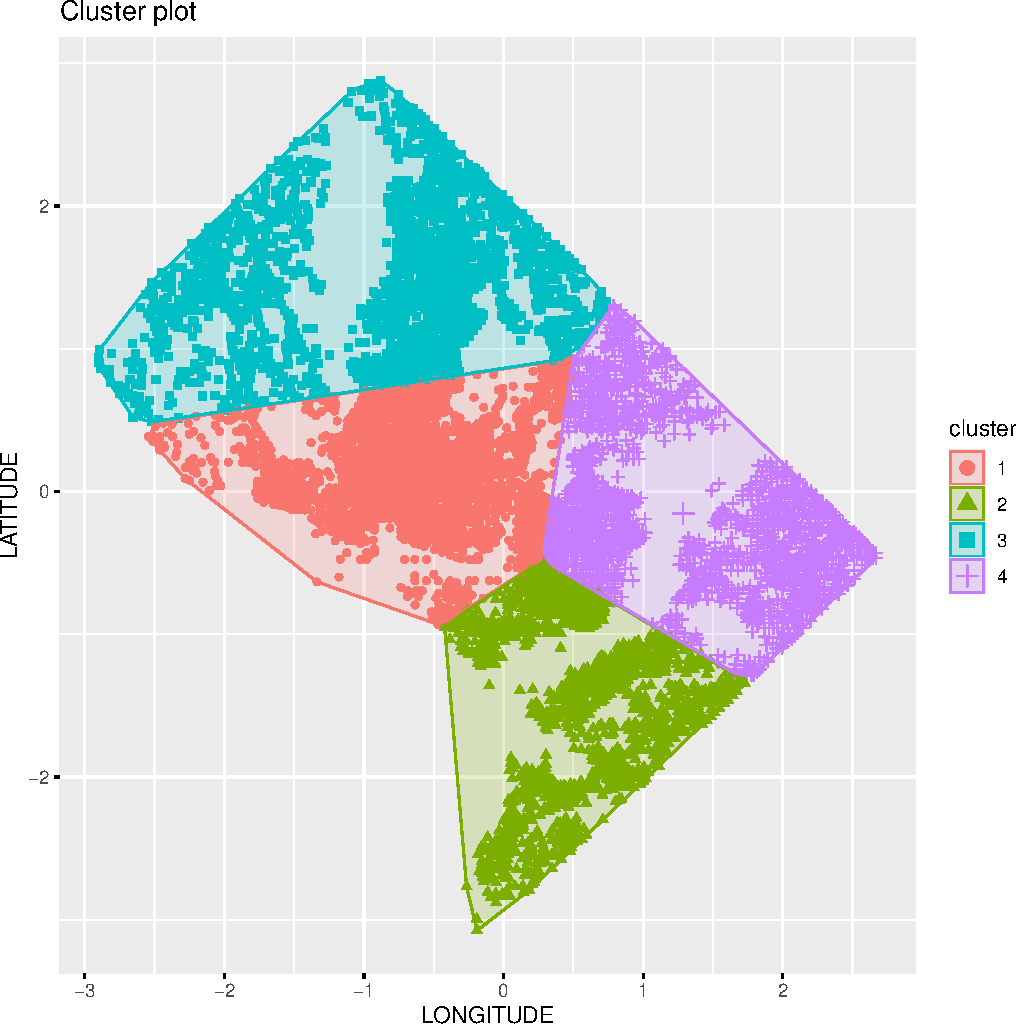
\includegraphics{./figures/unnamed-chunk-4-1} \end{center}

\begin{center}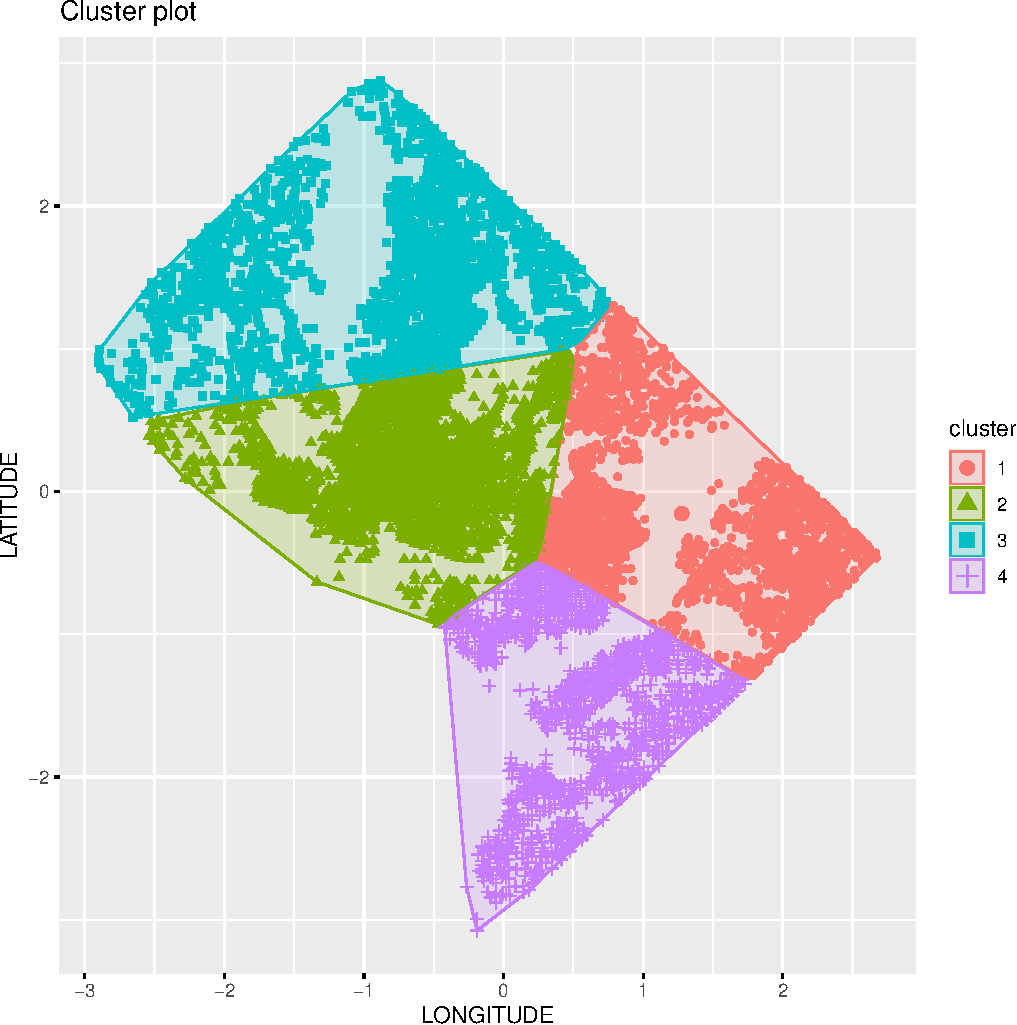
\includegraphics{./figures/unnamed-chunk-4-2} \end{center}

\begin{table}[H]
\centering
\resizebox{\ifdim\width>\linewidth\linewidth\else\width\fi}{!}{
\begin{tabular}[t]{r|l|r}
\hline
clusters & OFFENSE & count\\
\hline
1 & THEFT/OTHER & 2852\\
\hline
1 & THEFT F/AUTO & 1943\\
\hline
1 & MOTOR VEHICLE THEFT & 873\\
\hline
1 & ASSAULT W/DANGEROUS WEAPON & 669\\
\hline
1 & ROBBERY & 644\\
\hline
1 & BURGLARY & 402\\
\hline
1 & SEX ABUSE & 86\\
\hline
1 & HOMICIDE & 42\\
\hline
1 & ARSON & 2\\
\hline
2 & THEFT/OTHER & 6949\\
\hline
2 & THEFT F/AUTO & 4855\\
\hline
2 & ROBBERY & 646\\
\hline
2 & MOTOR VEHICLE THEFT & 608\\
\hline
2 & BURGLARY & 451\\
\hline
2 & ASSAULT W/DANGEROUS WEAPON & 420\\
\hline
2 & SEX ABUSE & 109\\
\hline
2 & HOMICIDE & 10\\
\hline
3 & THEFT/OTHER & 2132\\
\hline
3 & THEFT F/AUTO & 2034\\
\hline
3 & MOTOR VEHICLE THEFT & 404\\
\hline
3 & ROBBERY & 344\\
\hline
3 & BURGLARY & 283\\
\hline
3 & ASSAULT W/DANGEROUS WEAPON & 206\\
\hline
3 & SEX ABUSE & 35\\
\hline
3 & HOMICIDE & 13\\
\hline
3 & ARSON & 1\\
\hline
4 & THEFT/OTHER & 2531\\
\hline
4 & THEFT F/AUTO & 1424\\
\hline
4 & ASSAULT W/DANGEROUS WEAPON & 556\\
\hline
4 & ROBBERY & 535\\
\hline
4 & MOTOR VEHICLE THEFT & 522\\
\hline
4 & BURGLARY & 394\\
\hline
4 & SEX ABUSE & 67\\
\hline
4 & HOMICIDE & 50\\
\hline
4 & ARSON & 2\\
\hline
\end{tabular}}
\end{table}

\section{Conclusion}\label{conclusion}

This research project so far was set out to investigate the crime report
patterns in Washington D.C. based on the type of offenses, location, and
time. Based on the analysis, we were able to conclude for now that the
majority of offenses reported in Washington D.C. involved theft, and
that the majority of offenses reported were done during the Evening
Shift. I do believe that we would've had slightly better results on our
tables and plots if the data set didn't have so many missing values. In
the future, if I were to approach a similar task of investigating
something with data, I would prioritize handling missing values with
care.

\section{Appendix A: R Code}\label{appendix-a-r-code}

\subsection{Code for table 1:
appendix-load-data-n-table}\label{code-for-table-1-appendix-load-data-n-table}

\begin{Shaded}
\begin{Highlighting}[]
\CommentTok{\# We first read in the crime\_incidents csv file and store it as a data frame}
\NormalTok{crime\_incidents\_df }\OtherTok{\textless{}{-}} \FunctionTok{read.csv}\NormalTok{(}\StringTok{"Crime\_Incidents\_in\_2017.csv"}\NormalTok{)}

\CommentTok{\# We make a new column called "Month", and extract the month from the REPORT\_DAT variable }
\CommentTok{\# and place in the Month column}
\NormalTok{crime\_incidents\_df}\SpecialCharTok{$}\NormalTok{Month }\OtherTok{\textless{}{-}} \FunctionTok{month}\NormalTok{(crime\_incidents\_df}\SpecialCharTok{$}\NormalTok{REPORT\_DAT, }\AttributeTok{label =} \ConstantTok{TRUE}\NormalTok{)}

\CommentTok{\# We create an entirely new table that summarizes the months and offenses together}
\NormalTok{wide\_summary\_table }\OtherTok{\textless{}{-}} \FunctionTok{pivot\_wider}\NormalTok{(}\FunctionTok{summarize}\NormalTok{(}\FunctionTok{group\_by}\NormalTok{(crime\_incidents\_df, Month, OFFENSE), }
                                       \AttributeTok{Total =} \FunctionTok{n}\NormalTok{()), }
                             \AttributeTok{names\_from =}\NormalTok{ OFFENSE, }\AttributeTok{values\_from =}\NormalTok{ Total, }\AttributeTok{values\_fill =} \DecValTok{0}\NormalTok{)}

\CommentTok{\# We use kable() to give the table a better format}
\FunctionTok{kable}\NormalTok{(wide\_summary\_table, }\AttributeTok{caption =} \StringTok{"Total Amount of Crimes Reported Each Month per Offense"}\NormalTok{)}
\end{Highlighting}
\end{Shaded}

\subsection{Code for bar-graph:
appendix-plot-bar-graph}\label{code-for-bar-graph-appendix-plot-bar-graph}

\begin{Shaded}
\begin{Highlighting}[]
\CommentTok{\# We use pivot\_longer() to create a new data frame with the variables month, Offenses, }
\CommentTok{\# and Number of Crimes reported for those offenses.}
\NormalTok{long\_summary\_table }\OtherTok{\textless{}{-}} \FunctionTok{pivot\_longer}\NormalTok{(wide\_summary\_table, }
                                   \AttributeTok{col =} \SpecialCharTok{{-}}\NormalTok{Month, }
                                   \AttributeTok{names\_to =} \StringTok{"Offenses"}\NormalTok{, }
                                   \AttributeTok{values\_to =} \StringTok{"Number\_of\_Times\_Crimes\_Reported"}\NormalTok{)}

\CommentTok{\# We use ggplot() and geom\_bar() to create a bar graph of the number of crimes reported }
\CommentTok{\# for each crime in each month.}
\CommentTok{\# We use aes() to give the plot object x, y and fill values and geom\_bar() to make }
\CommentTok{\# the plot object a bar plot object.}
\FunctionTok{ggplot}\NormalTok{(}\AttributeTok{data =}\NormalTok{ long\_summary\_table, }
       \FunctionTok{aes}\NormalTok{(}\AttributeTok{x =}\NormalTok{ Month, }\AttributeTok{y =}\NormalTok{ Number\_of\_Times\_Crimes\_Reported, }\AttributeTok{fill =}\NormalTok{ Offenses)) }\SpecialCharTok{+} 
  \FunctionTok{geom\_bar}\NormalTok{(}\AttributeTok{stat =} \StringTok{"identity"}\NormalTok{) }\SpecialCharTok{+} 
  \FunctionTok{labs}\NormalTok{(}\AttributeTok{title =} \StringTok{"Crimes Reported Each Month and Offense"}\NormalTok{,}
       \AttributeTok{x =} \StringTok{"Month"}\NormalTok{,}
       \AttributeTok{y =} \StringTok{"Number of Crimes Reported"}\NormalTok{)}
\end{Highlighting}
\end{Shaded}

\subsection{Code for table 2:
appendix-load-univariate-table}\label{code-for-table-2-appendix-load-univariate-table}

\begin{Shaded}
\begin{Highlighting}[]
\CommentTok{\# We use summarize() to get the summary statistic of the longitude and latitude }
\CommentTok{\# variables, then we store those values onto a table.}
\NormalTok{univariate\_summary\_table }\OtherTok{\textless{}{-}} \FunctionTok{summarize}\NormalTok{(crime\_incidents\_df,}
                                      \AttributeTok{longitude\_min =} \FunctionTok{min}\NormalTok{(LONGITUDE),}
                                      \AttributeTok{longitude\_max =} \FunctionTok{max}\NormalTok{(LONGITUDE),}
                                      \AttributeTok{longitude\_mean =} \FunctionTok{mean}\NormalTok{(LONGITUDE),}
                                      \AttributeTok{longitude\_median =} \FunctionTok{median}\NormalTok{(LONGITUDE),}
                                      \AttributeTok{longitude\_sd =} \FunctionTok{sd}\NormalTok{(LONGITUDE),}
                                      \AttributeTok{latitude\_min =} \FunctionTok{min}\NormalTok{(LATITUDE),}
                                      \AttributeTok{latitude\_max =} \FunctionTok{max}\NormalTok{(LATITUDE),}
                                      \AttributeTok{latitude\_mean =} \FunctionTok{mean}\NormalTok{(LATITUDE),}
                                      \AttributeTok{latitude\_median =} \FunctionTok{median}\NormalTok{(LATITUDE),}
                                      \AttributeTok{latitude\_sd =} \FunctionTok{sd}\NormalTok{(LATITUDE)) }

\CommentTok{\# Next we use pivot\_longer to make the table horizontal, make it more readable.}
\NormalTok{univariate\_summary\_table }\OtherTok{\textless{}{-}} \FunctionTok{pivot\_longer}\NormalTok{(univariate\_summary\_table, }\FunctionTok{everything}\NormalTok{())}

\CommentTok{\# After we use kable() to properly format the table and give the table a caption.}
\FunctionTok{kable}\NormalTok{(univariate\_summary\_table, }\AttributeTok{caption =} \StringTok{"Univariate Summary Table of Longitude and Latitude"}\NormalTok{)}
\end{Highlighting}
\end{Shaded}

\subsection{Code for scatter plot:
appendix-plot-scatterplot}\label{code-for-scatter-plot-appendix-plot-scatterplot}

\begin{Shaded}
\begin{Highlighting}[]
\CommentTok{\# We use ggplot() and geom\_point() to create the plot object and make the plot object a scatter plot.}
\CommentTok{\# We use aes() to give the plot object data to plot and labs() to give the plot labels.}
\FunctionTok{ggplot}\NormalTok{(crime\_incidents\_df, }\FunctionTok{aes}\NormalTok{(}\AttributeTok{x =}\NormalTok{ LONGITUDE, }\AttributeTok{y =}\NormalTok{ LATITUDE)) }\SpecialCharTok{+} \FunctionTok{geom\_point}\NormalTok{(}\FunctionTok{aes}\NormalTok{(}\AttributeTok{color =}\NormalTok{ OFFENSE)) }\SpecialCharTok{+}
  \FunctionTok{labs}\NormalTok{(}\AttributeTok{title =} \StringTok{"Crime Locations in DC"}\NormalTok{, }
       \AttributeTok{x =} \StringTok{"Longitude"}\NormalTok{,}
       \AttributeTok{y =} \StringTok{"Latitude"}\NormalTok{)}
\end{Highlighting}
\end{Shaded}

\subsection{Code for Table 3:
appendix-load-bivariate-summary-table}\label{code-for-table-3-appendix-load-bivariate-summary-table}

\begin{Shaded}
\begin{Highlighting}[]
\CommentTok{\# We extract the hour from the entries in the variable "REPORT\_DAT" and store those entries }
\CommentTok{\# in a new Hour variable.}
\NormalTok{crime\_incidents\_df}\SpecialCharTok{$}\NormalTok{Hour }\OtherTok{\textless{}{-}} \FunctionTok{hour}\NormalTok{(crime\_incidents\_df}\SpecialCharTok{$}\NormalTok{REPORT\_DAT)}

\CommentTok{\# We calculate the summary statistics of the Hour per Shift, this is by using summarize(),}
\CommentTok{\# group\_by(), which groups the data set itself and the SHIFT variable, then summarize() }
\CommentTok{\# produces the results for the data set and SHIFT variable. We calculate the the summary }
\CommentTok{\# statistics for the SHIFT variable.}
\NormalTok{summary\_table }\OtherTok{\textless{}{-}} \FunctionTok{summarize}\NormalTok{(}\FunctionTok{group\_by}\NormalTok{(crime\_incidents\_df, SHIFT), }
                           \AttributeTok{min\_hour =} \FunctionTok{min}\NormalTok{(Hour),}
                           \AttributeTok{lower\_quantile\_hour =} \FunctionTok{quantile}\NormalTok{(Hour, }\FloatTok{0.25}\NormalTok{),}
                           \AttributeTok{median\_hour =} \FunctionTok{median}\NormalTok{(Hour),}
                           \AttributeTok{upper\_quantile\_hour =} \FunctionTok{quantile}\NormalTok{(Hour, }\FloatTok{0.75}\NormalTok{),}
                           \AttributeTok{max\_hour =} \FunctionTok{max}\NormalTok{(Hour),}
                           \AttributeTok{mean\_hour =} \FunctionTok{mean}\NormalTok{(Hour),}
                           \AttributeTok{sd\_hour =} \FunctionTok{sd}\NormalTok{(Hour))}

\CommentTok{\# We use kable() to properly format the table we created and give it a caption}
\FunctionTok{kable}\NormalTok{(summary\_table, }\AttributeTok{caption =} \StringTok{"Bivariate Summary Table of Hours per Shift"}\NormalTok{)}
\end{Highlighting}
\end{Shaded}

\subsection{Code for boxplot:
appendix-box-plot}\label{code-for-boxplot-appendix-box-plot}

\begin{Shaded}
\begin{Highlighting}[]
\CommentTok{\# We use ggplot() and geom\_boxplot() to create a plot object with the SHIFT and hour variables}
\CommentTok{\# from the data set. }
\CommentTok{\# Then we use geom\_boxplot() to make the plot object a boxplot object with its labels included.}
\FunctionTok{ggplot}\NormalTok{(crime\_incidents\_df,}
       \FunctionTok{aes}\NormalTok{(}\AttributeTok{x =}\NormalTok{ SHIFT, }
           \AttributeTok{y =}\NormalTok{ Hour, }
           \AttributeTok{color =}\NormalTok{ SHIFT)) }\SpecialCharTok{+}
  \FunctionTok{geom\_boxplot}\NormalTok{() }\SpecialCharTok{+} 
  \FunctionTok{labs}\NormalTok{(}\AttributeTok{title =} \StringTok{"Crimes Reported Hour Distribution per Shift"}\NormalTok{,}
       \AttributeTok{x =} \StringTok{"Police Shift when Crime was reported"}\NormalTok{,}
       \AttributeTok{y =} \StringTok{"Hour of the report"}\NormalTok{)}
\end{Highlighting}
\end{Shaded}

\subsection{Code for Table 4:
appendix-load-bivariate-summary-table-2}\label{code-for-table-4-appendix-load-bivariate-summary-table-2}

\begin{Shaded}
\begin{Highlighting}[]
\CommentTok{\# We use summarize() and group() and include the crime data set, variable Month and Shift }
\CommentTok{\# to create a table that contains}
\CommentTok{\# the information of the amount of crimes reported for each type of offense for each month.}
\NormalTok{month\_shift\_trend }\OtherTok{\textless{}{-}} \FunctionTok{summarize}\NormalTok{(}\FunctionTok{group\_by}\NormalTok{(crime\_incidents\_df, Month, SHIFT), }\AttributeTok{n =} \FunctionTok{n}\NormalTok{())}

\CommentTok{\# We use summarize() and group() and include the crime data set, variable n and Shift to }
\CommentTok{\# find the summary statistics of the number of crimes reported per shift.}
\NormalTok{summary\_table }\OtherTok{\textless{}{-}} \FunctionTok{summarize}\NormalTok{(}\FunctionTok{group\_by}\NormalTok{(month\_shift\_trend, SHIFT),}
                           \AttributeTok{min\_n =} \FunctionTok{min}\NormalTok{(n),}
                           \AttributeTok{max\_n =} \FunctionTok{max}\NormalTok{(n),}
                           \AttributeTok{mean\_n =} \FunctionTok{mean}\NormalTok{(n),}
                           \AttributeTok{median\_n =} \FunctionTok{median}\NormalTok{(n),}
                           \AttributeTok{sd\_n =} \FunctionTok{sd}\NormalTok{(n))}

\CommentTok{\# We use kable() to properly format the table we created and give it a caption}
\FunctionTok{kable}\NormalTok{(summary\_table, }\AttributeTok{caption =} \StringTok{"Bivariate Summary Table of Hours per Shift"}\NormalTok{)}
\end{Highlighting}
\end{Shaded}

\subsection{Code for plot-trend-line:
appendix-plot-trend-line}\label{code-for-plot-trend-line-appendix-plot-trend-line}

\begin{Shaded}
\begin{Highlighting}[]
\CommentTok{\# We use ggplot() along with the month\_shift\_trend data set, variables Month and }
\CommentTok{\# n (number of crimes committed for each month) to create a trend line graph. }
\CommentTok{\# labs() is used to give the graph its labels etc.}
\FunctionTok{ggplot}\NormalTok{(month\_shift\_trend, }
       \FunctionTok{aes}\NormalTok{(}\AttributeTok{x =}\NormalTok{ Month,}
           \AttributeTok{y =}\NormalTok{ n,}
           \AttributeTok{color =}\NormalTok{ SHIFT,}
           \AttributeTok{group =}\NormalTok{ SHIFT)) }\SpecialCharTok{+}
  \FunctionTok{geom\_line}\NormalTok{() }\SpecialCharTok{+} 
  \FunctionTok{labs}\NormalTok{(}\AttributeTok{title =} \StringTok{"Crime Month Trend by Shift"}\NormalTok{,}
       \AttributeTok{x =} \StringTok{"Month"}\NormalTok{,}
       \AttributeTok{y =} \StringTok{"Number of Crimes Reported"}\NormalTok{)}
\end{Highlighting}
\end{Shaded}


\end{document}
